\chapter{Results}
\label{ch_results}

These are the results I found from my investigation.

Present your results in a suitable format using tables and graphs where necessary. Remember to refer
to them in text and caption them properly.


\section{Simulation Results}


\section{Experimental Results}

\subsection{Focal Length of Lens}

The measured focal length of the lens was measured to be 53mm. Figure \ref{fig:focal_length_experiemnt_result} shows the focused point formed after adjusting the lens to 5.3cm above the working surface.

\begin{figure}[H]
	\centering
	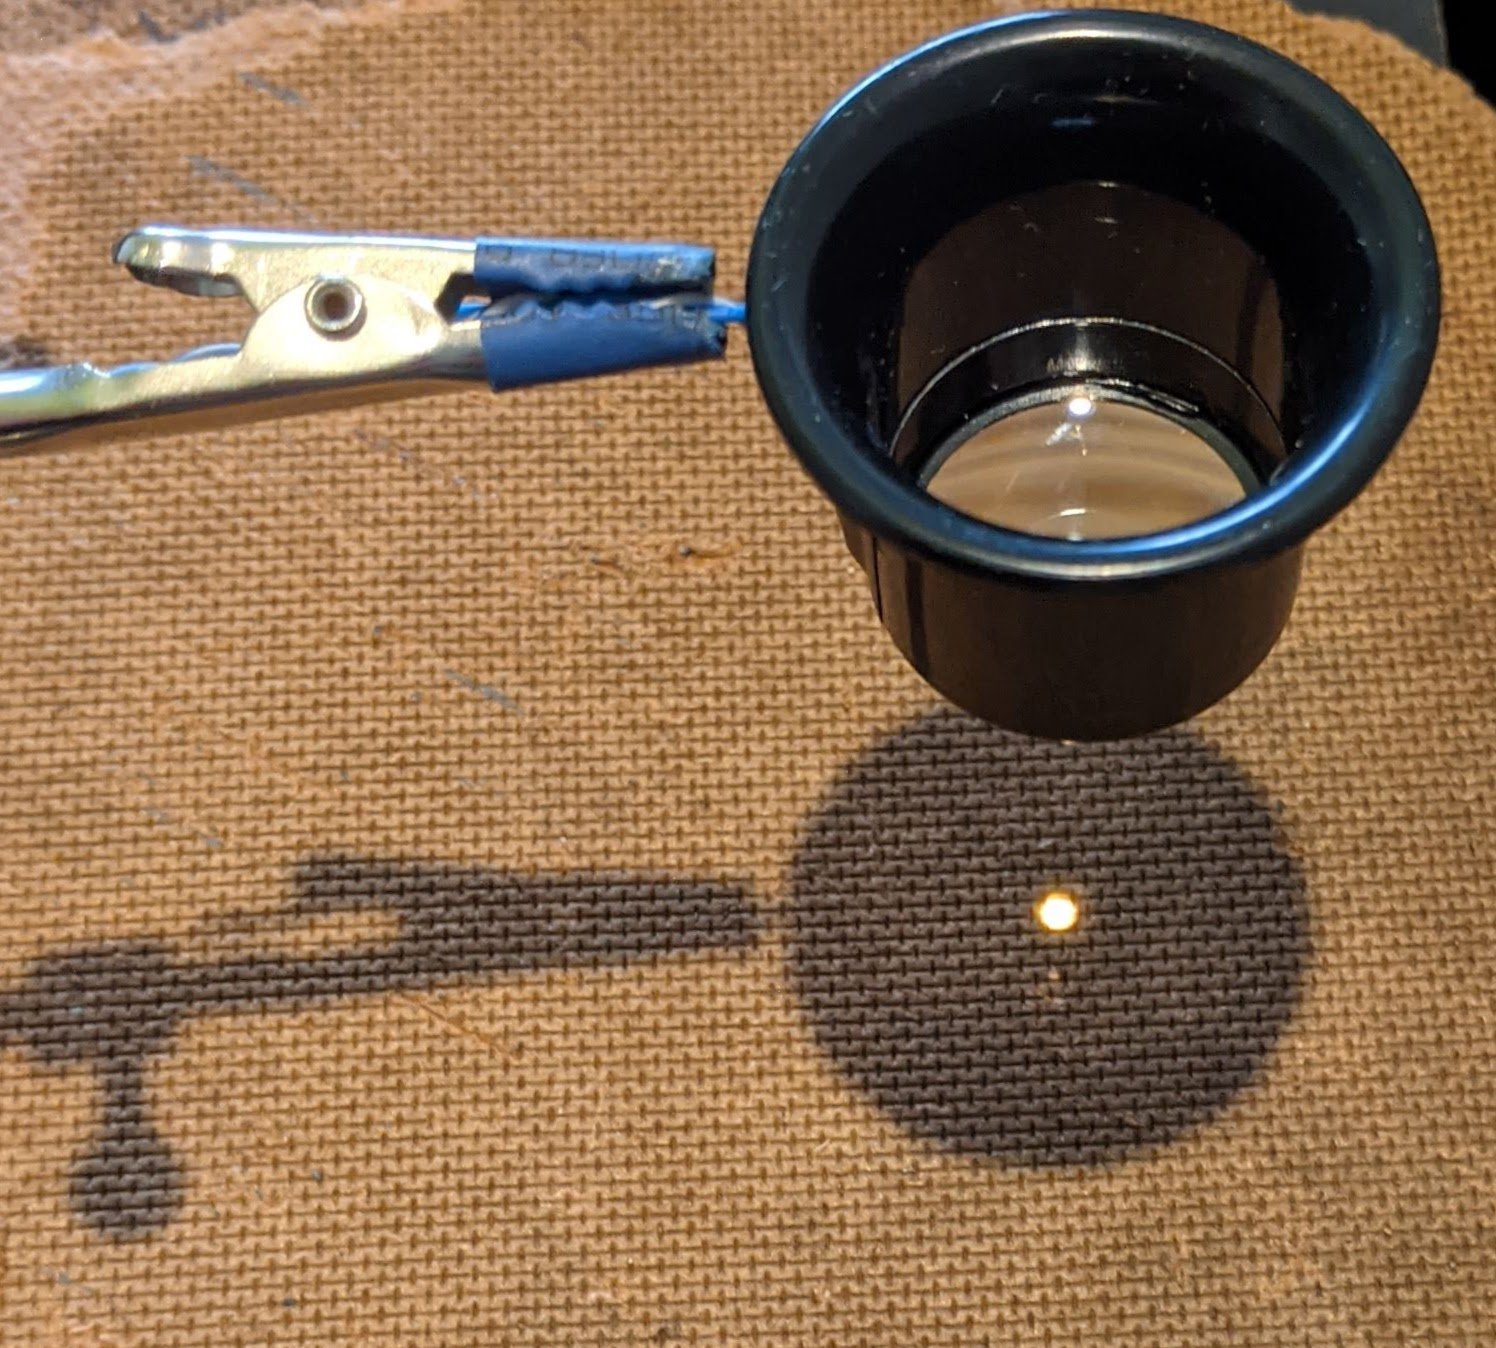
\includegraphics[width=.6\linewidth]{figures/results/focal_length_result.jpg}
	\captionof{figure}{Focal Length Experiemnt}
	\label{fig:focal_length_experiemnt_result}
\end{figure}


\subsection{Light Focus System}

Table \ref{label} below shows the beam spot size vs distance for the IR and warm-white power LEDs.

%table here

\subsection{Goertzel Filter Optimization}

\begin{figure}[H]
	\centering
	\begin{minipage}{.4\textwidth}
		\centering
		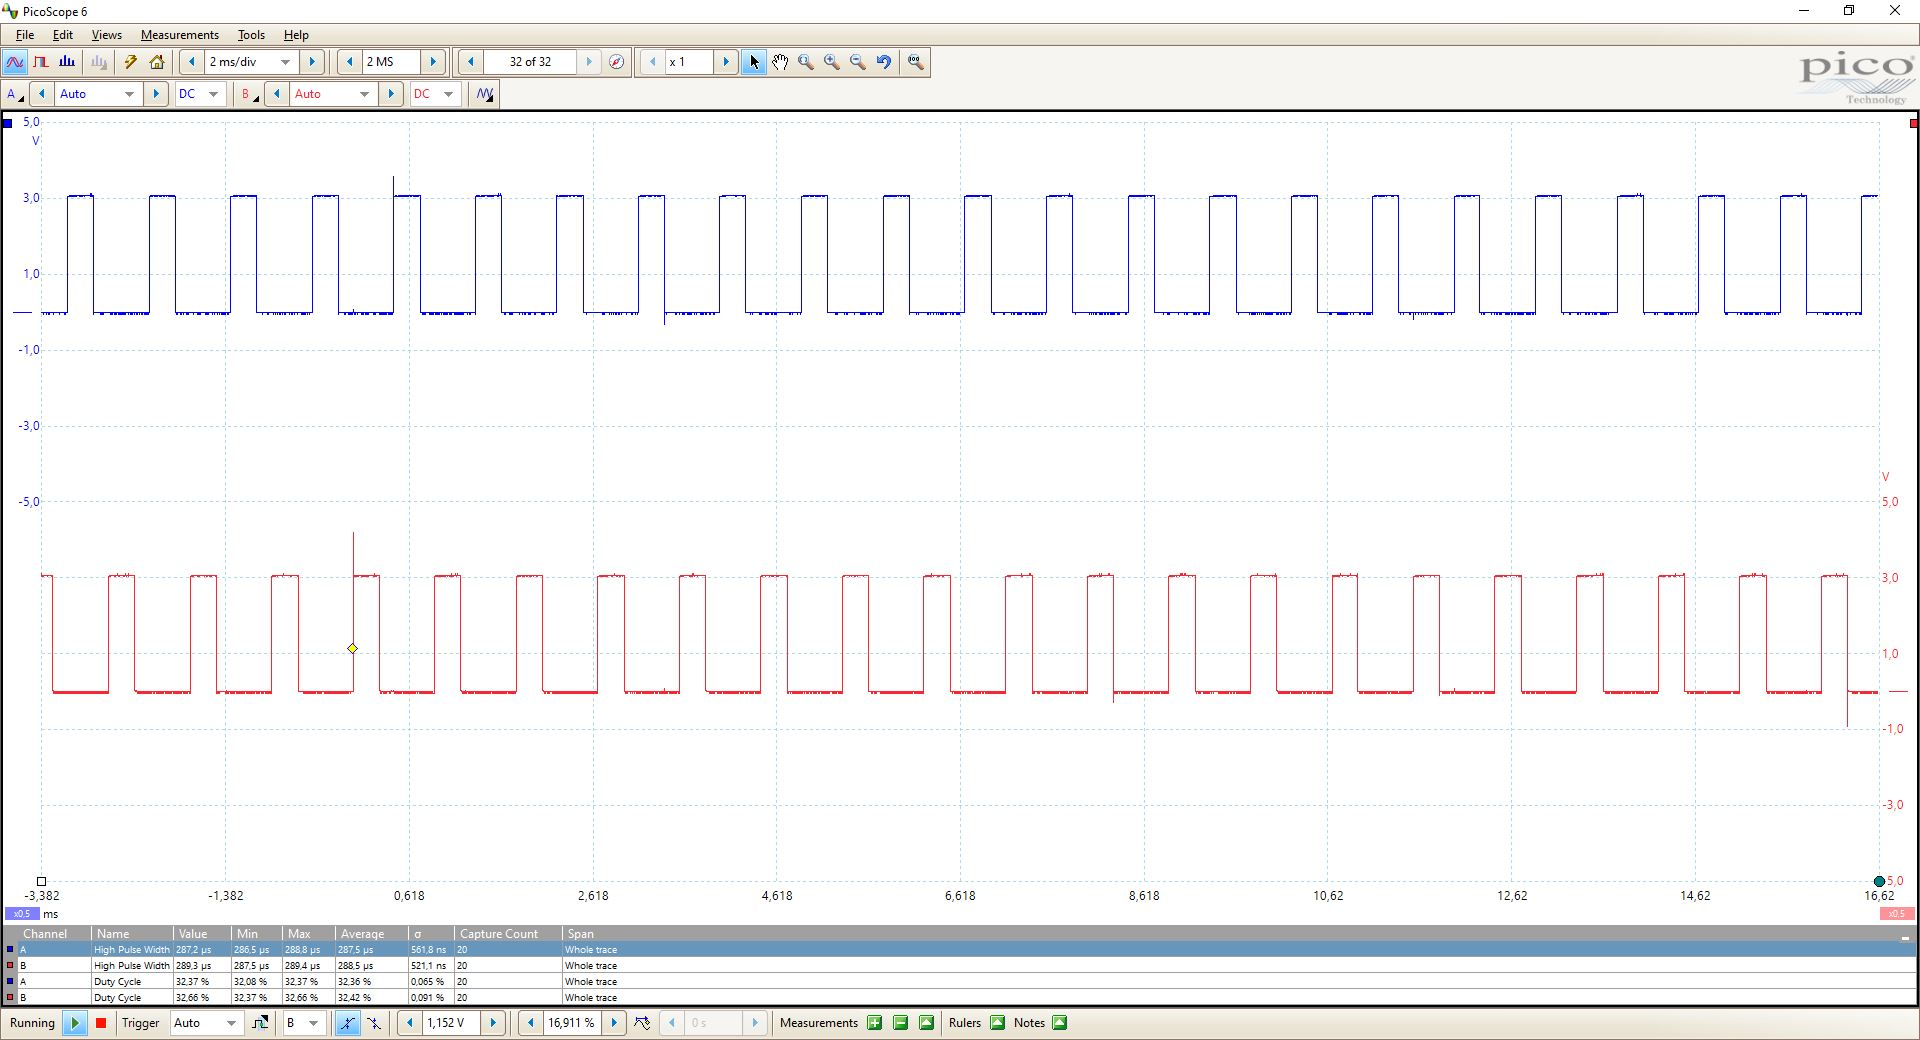
\includegraphics[width=0.9\linewidth]{figures/results/goertzel_filter_speed/16nu.JPG}
		\captionof{figure}{Scope Reading for unoptimized goertzel with $N = 16$}
		\label{fig:goertzel_speed_scope_screenshot}
	\end{minipage}%
	\hspace{.1\textwidth}
	\begin{minipage}{.4\textwidth}
		\begin{table}[H]
			\begin{tabular}{ccc}
				\hline
				\textbf{N} & \textbf{\begin{tabular}[c]{@{}c@{}}Unoptimized\\ ($\mu S$)\end{tabular}} & \textbf{\begin{tabular}[c]{@{}c@{}}Optimized\\ ($\mu S$)\end{tabular}} \\ \hline
				4 & 96.46 & 61.15 \\ \hline
				8 & 160.3 & 98.35 \\ \hline
				16 & 287.5 & 171.9 \\ \hline
				32 & 547.2 & 323.9 \\ \hline
				64 & 1059 & 621.1
			\end{tabular}
			\captionof{table}{Compiled results for goertzel speed experiemnt}
			\label{tbl:goertzel_speed_results}
		\end{table}
	\end{minipage}
\end{figure}

\begin{figure}[H]
	\centering
	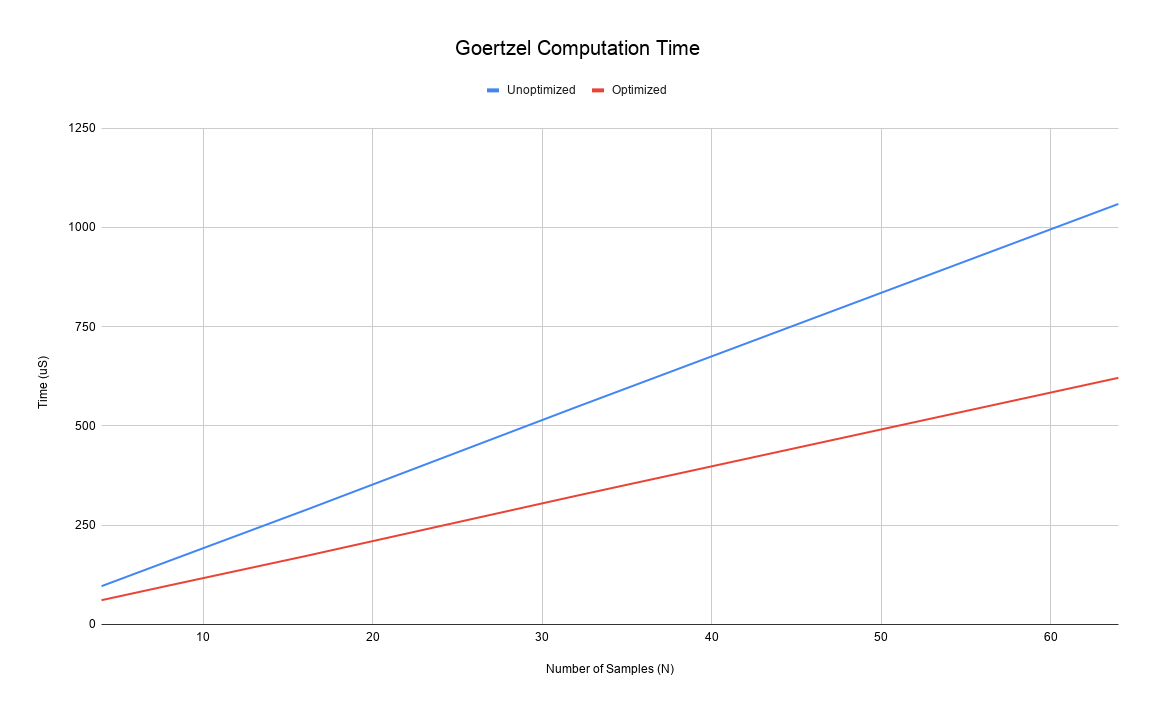
\includegraphics[width=\linewidth]{figures/results/goertzel_filter_speed/goertzel_computation_time.png}
	\captionof{figure}{Goertzel computation time versus sample set size}
	\label{fig:goertzel_computation_time}
\end{figure}
